\documentclass{article}

\usepackage[left=1cm, right=1cm, top=1cm, bottom=2cm]{geometry}
\usepackage{listingsutf8}
\usepackage[utf8]{inputenc}
\usepackage[T1]{fontenc}
\usepackage{xcolor}
\usepackage{amssymb}
\usepackage{stmaryrd}
\usepackage{amsmath}
\usepackage{mathtools}
\usepackage{parskip}
\usepackage{xypic}
\usepackage{tikz}
\usepackage{svg}
\usepackage{pdfpages}
\usepackage{hyperref}
\usepackage{titlesec}
\usepackage[normalem]{ulem}
\usepackage{graphicx}

\usetikzlibrary{shapes.callouts}

\DeclarePairedDelimiter\ceil{\lceil}{\rceil}
\DeclarePairedDelimiter\floor{\lfloor}{\rfloor}

\newcommand{\schem}[3]
{
	\begin{figure}[ht]
		\centering
		\textbf{#1}\par\medskip
		\includegraphics[scale=#3]{figures/figure#2}
		\caption{}
	\end{figure}
}

\lstset{inputencoding=utf8/latin1}

\lstnewenvironment{case}
{
	\renewcommand\lstlistingname{Case}
	\lstset{style = mystyle}
}{}

\newcommand{\code}[1]{\lstinline[style = mystyle]{#1}}

\lstset
{
    frame=tb,
    tabsize=4,
    showstringspaces=false,
    numbers=left,
    commentstyle=\color{gray},
    keywordstyle=\color{blue},
    stringstyle=\color{red},
		literate=
		{á}{{\'a}}1 {é}{{\'e}}1 {í}{{\'i}}1 {ó}{{\'o}}1 {ú}{{\'u}}1
    {Á}{{\'A}}1 {É}{{\'E}}1 {Í}{{\'I}}1 {Ó}{{\'O}}1 {Ú}{{\'U}}1
    {à}{{\`a}}1 {è}{{\`e}}1 {ì}{{\`i}}1 {ò}{{\`o}}1 {ù}{{\`u}}1
    {À}{{\`A}}1 {È}{{\'E}}1 {Ì}{{\`I}}1 {Ò}{{\`O}}1 {Ù}{{\`U}}1
    {ä}{{\"a}}1 {ë}{{\"e}}1 {ï}{{\"i}}1 {ö}{{\"o}}1 {ü}{{\"u}}1
    {Ä}{{\"A}}1 {Ë}{{\"E}}1 {Ï}{{\"I}}1 {Ö}{{\"O}}1 {Ü}{{\"U}}1
    {â}{{\^a}}1 {ê}{{\^e}}1 {î}{{\^i}}1 {ô}{{\^o}}1 {û}{{\^u}}1
    {Â}{{\^A}}1 {Ê}{{\^E}}1 {Î}{{\^I}}1 {Ô}{{\^O}}1 {Û}{{\^U}}1
    {œ}{{\oe}}1 {Œ}{{\OE}}1 {æ}{{\ae}}1 {Æ}{{\AE}}1 {ß}{{\ss}}1
    {ç}{{\c c}}1 {Ç}{{\c C}}1 {ø}{{\o}}1 {å}{{\r a}}1 {Å}{{\r A}}1
    {€}{{\EUR}}1 {£}{{\pounds}}1
}

\lstdefinestyle{mystyle}
{
    language = Caml,
		otherkeywords = {ref,;,decr,incr,false,true,raise,when,log,failwith,sin,cos,tan,mod,abs,exp,sqrt,tanh,int_of_float,float_of_int,int_of_float,unit,char_of_int,int_of_char},
}

\setcounter{secnumdepth}{5}

\titleformat{\paragraph}
{\normalfont\normalsize\bfseries}{\theparagraph}{1em}{}
\titlespacing*{\paragraph}
{0pt}{3.25ex plus 1ex minus .2ex}{1.5ex plus .2ex}

\begin{document}

	\obeylines

	\title{\vspace{-1.7cm}Option informatique: Devoir maison (Toussaint)\\
	\large Benjamin LOISON (MP*)
			\\22 octobre 2019}
	\date{}
	\maketitle

	\vspace{-2.3cm}\noindent\makebox[\linewidth]{\rule{\paperwidth}{0.4pt}}
	\vspace{4cm}\noindent\makebox[\linewidth]{\rule{\paperwidth}{0.4pt}}

	\section{Première partie}

		\setcounter{subsection}{16}
		\subsection{}

			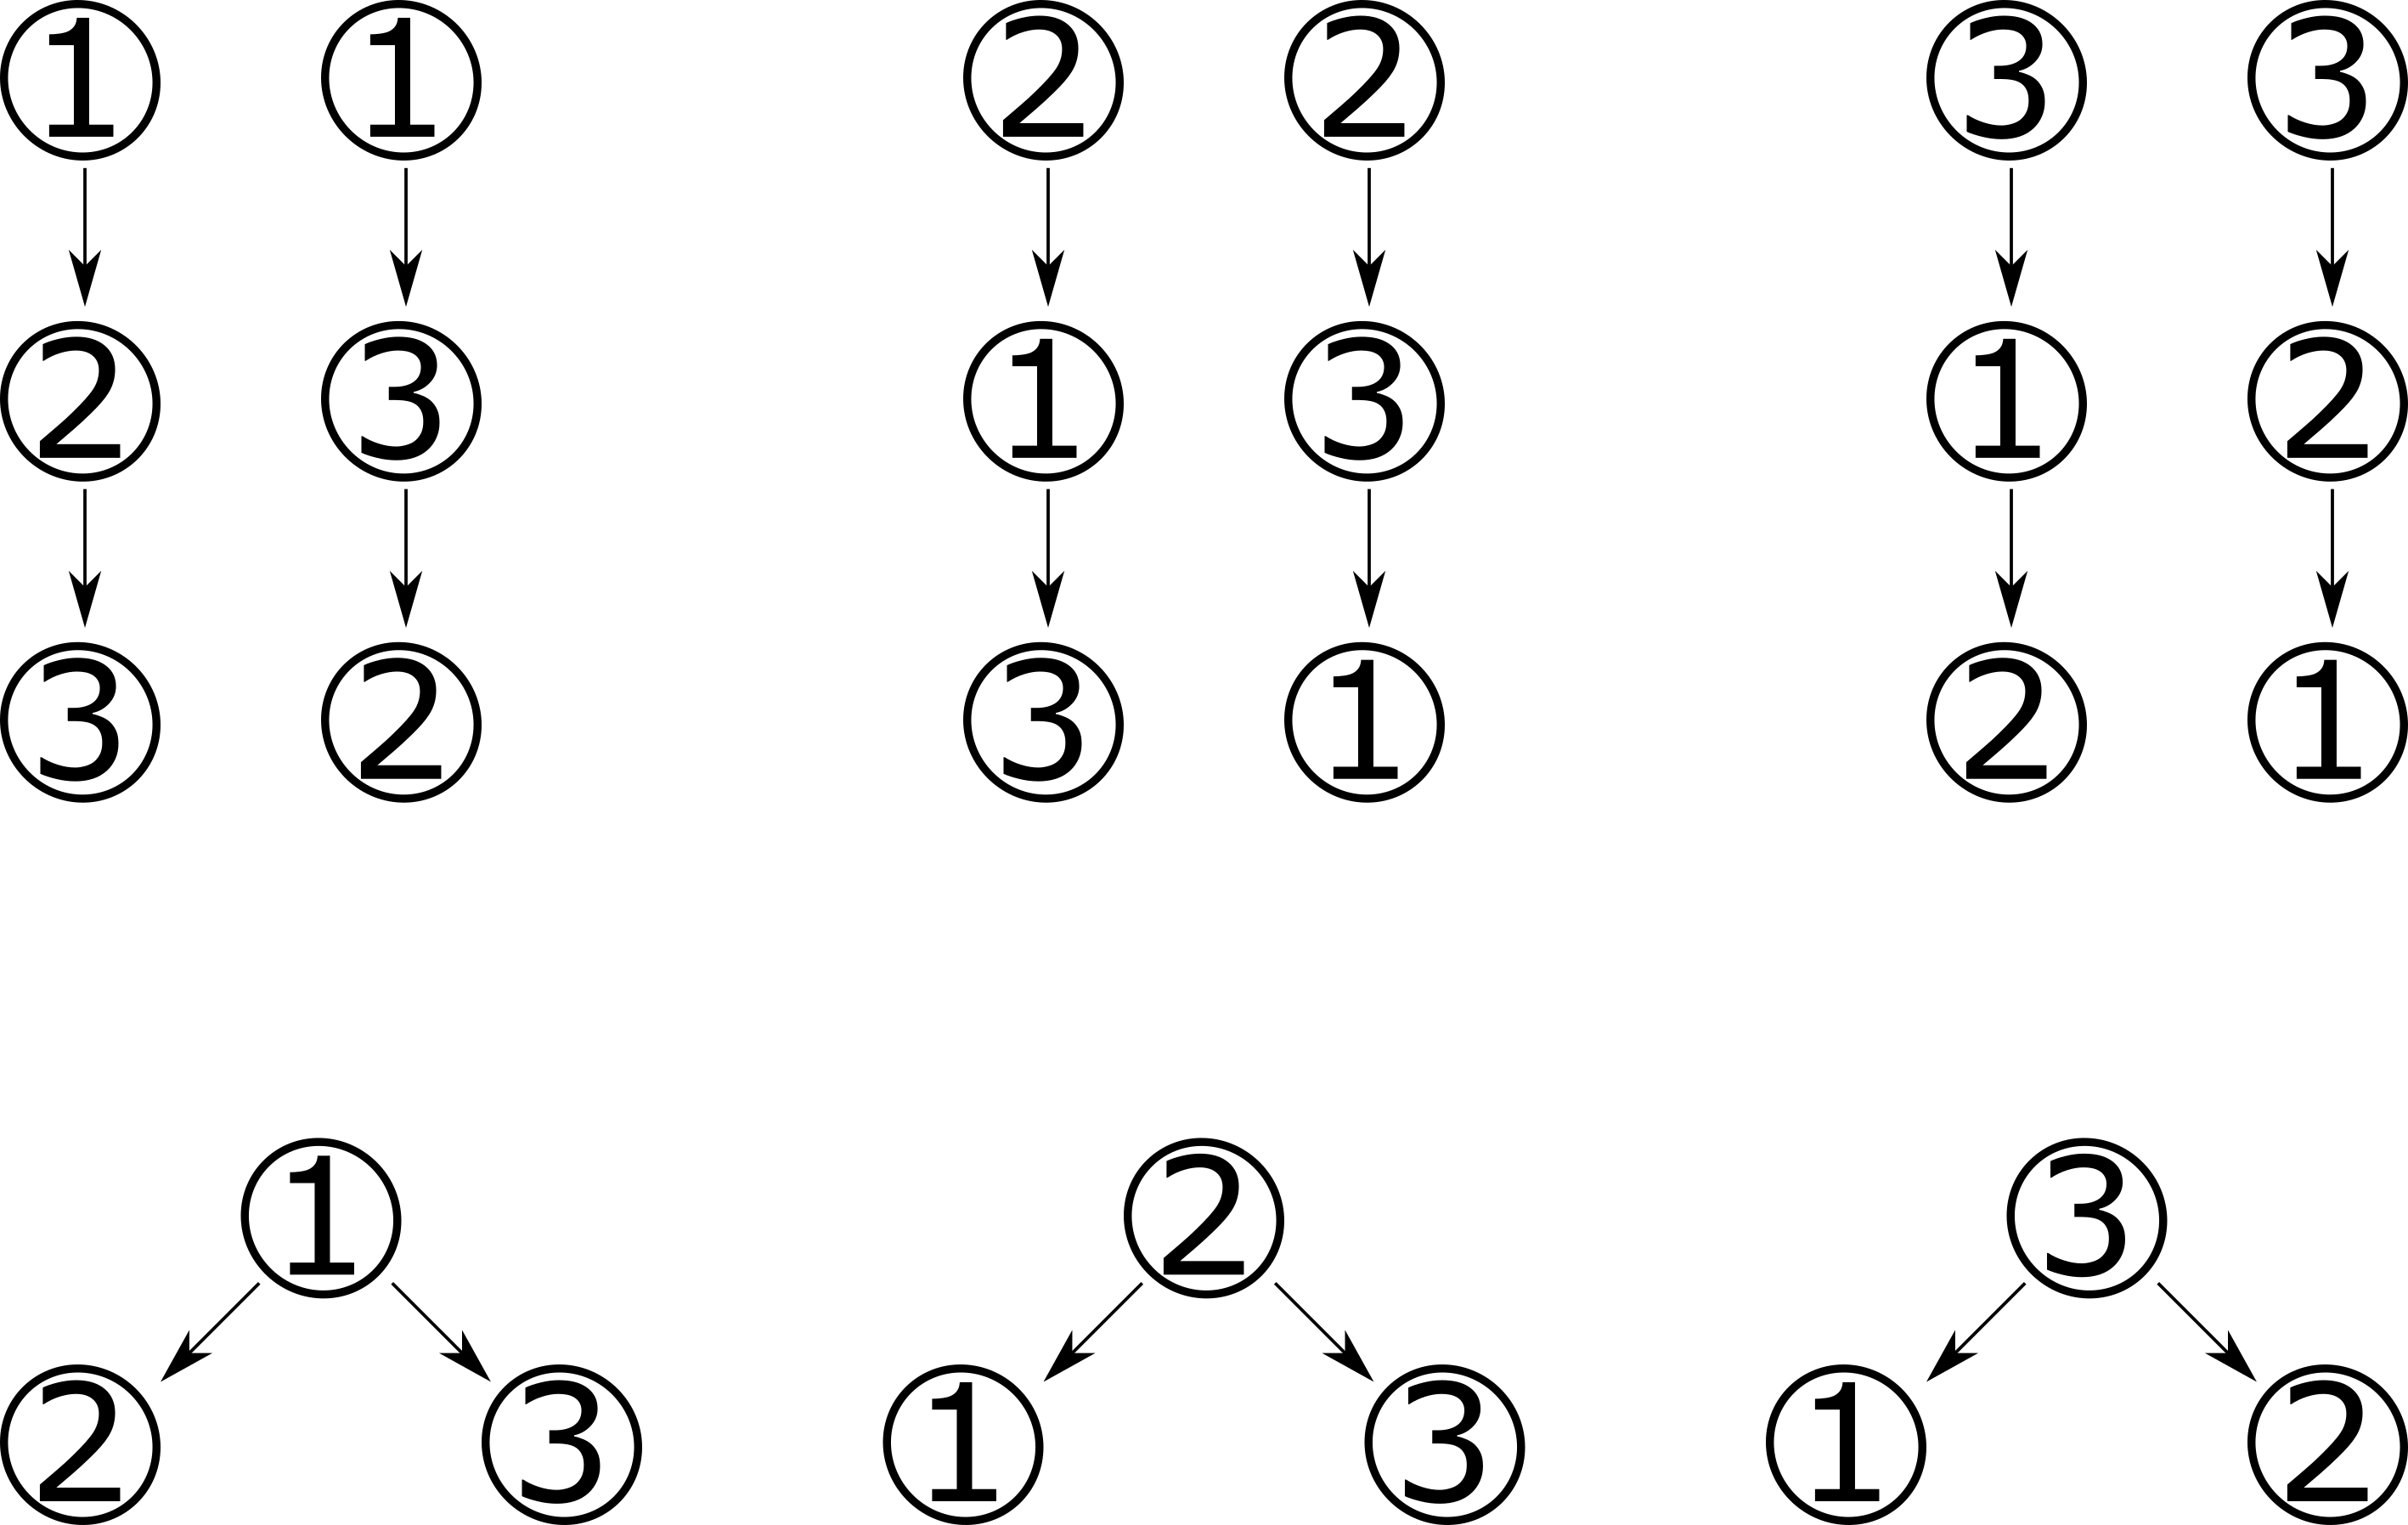
\includegraphics[scale=0.1]{IMG/PNG/17.png}

		\subsection{}
		
			\begin{case}
let calculer_peres racine fils freres =
	let peres = Array.make (Array.length fils) (-1) in
		let rec aux indice father =
			let child = fils.(indice) and brother = freres.(indice) in
			if (child <> -1) then (peres.(child) <- indice; aux child indice);
			if (brother <> -1) then (peres.(brother) <- father; aux brother father);
		in aux racine 0;
	peres;;
			\end{case}
		
		\subsection{}
		
			La fonction \code{calculer_peres} est linéaire en le nombre de noeuds de l'arbre considéré. % need justify ?
			
		\subsection{}
		
			\begin{case}
let calculer_arites fils freres =
	let rec aux indice = match freres.(indice) with
	| (-1) -> 1
	| f -> 1 + (aux f); in
	let n = Array.length fils in
		let arites = Array.make n 0 in
			for i = 0 to (n - 1) do
				if (fils.(i) <> (-1)) then
					arites.(i) <- (aux fils.(i));
			done;
	arites;;
			\end{case}
		
		\subsection{}
		
			La fonction \code{calculer_arites} est linéaire en le nombre de noeuds de l'arbre considéré.

		\subsection{}

			\begin{case}
let inserer table nb d =
	let rec aux i j = match (i + j + 1) / 2 with
	| k when j < i ->
		for i = (max 0 (nb - 1)) to k do
			table.(i + 1) <- table.(i);
		done;
		table.(k) <- d;
	| k when table.(k) > d -> aux (k + 1) j
	| k -> aux i (k - 1)
	in aux 0 (nb - 1);
	nb + 1;;
			\end{case}
			
		\subsection{}
		
			La fonction \code{inserer} est linéaire en le nombre d'entiers contenus dans le tableau trié considéré.
			
		\subsection{}
		
			Le codage de Prüfer de l'abre $A_3$ est: 9, 1, 6, 7, 1, 3, 7, 9, 9, 3.
			
		\subsection{}
		
			
			\begin{case}
let calculer_Prufer racine fils freres =
	let n = Array.length fils and
		peres = calculer_peres racine fils freres and
		arites = calculer_arites fils freres and
		feuillesIndex = ref 0 in
	let feuilles = Array.make n 0 and prufer = Array.make (n - 1) 0 in
	for i = n - 1 downto 0 do
		if arites.(i) = 0 then
		(	feuilles.(!feuillesIndex) <- i;
			incr feuillesIndex)
	done;
	for i = 0 to n - 2 do
		let noeud = feuilles.(!feuillesIndex - 1) in
		let pere = peres.(noeud) in
			decr feuillesIndex;
			prufer.(i) <- pere;
			arites.(pere) <- arites.(pere) - 1;
			if arites.(pere) = 0 then
				feuillesIndex := inserer feuilles !feuillesIndex pere;
	done;
	prufer;;
			\end{case}
		
		\subsection{}
		
			La fonction \code{calculer_Prufer} est quadratique en le nombre de noeuds de l'arbre considéré.
		
	\section{Seconde partie}
			
		\setcounter{subsection}{26}
		\subsection{}

			Chaque occurence d'une étiquette dans le codage de Prüfer est synonyme de l'existence d'un fils de cette étiquette, d'où:
		
			\begin{case}
let calculer_arites_par_Prufer prufer =
	let n = Array.length prufer in
	let arites = Array.make (n + 1) 0 in
	for i = 0 to n - 1 do
		print_int i;
		let j = prufer.(i) in
		arites.(j) <- arites.(j) + 1
	done;
	arites;;
			\end{case}
		
		\subsection{}
		
			2 est le dernier élément du codage de Prüfer c'est donc la racine.
			L'arbre étant consécutivement étiqueté et 1 n'apparaît pas dans le codage de Prüfer donc 1 est une feuille et est fils de 2.
			0 est le plus petit élément de $\llbracket0; 5\rrbracket$, l'unique occurence de 0 dans le codage de Prüfer et la présence de la séquence 0, 2 dans le codage de Prüfer montre que 0 est fils de 2.
			5 et 4 sont des feuilles car ils n'apparaissent pas dans le codage de Prüfer.
			3 est le père de 4 car 4 est la plus petite feuille parmi 4 et 5.
			
			D'où l'arbre suivant:
		
			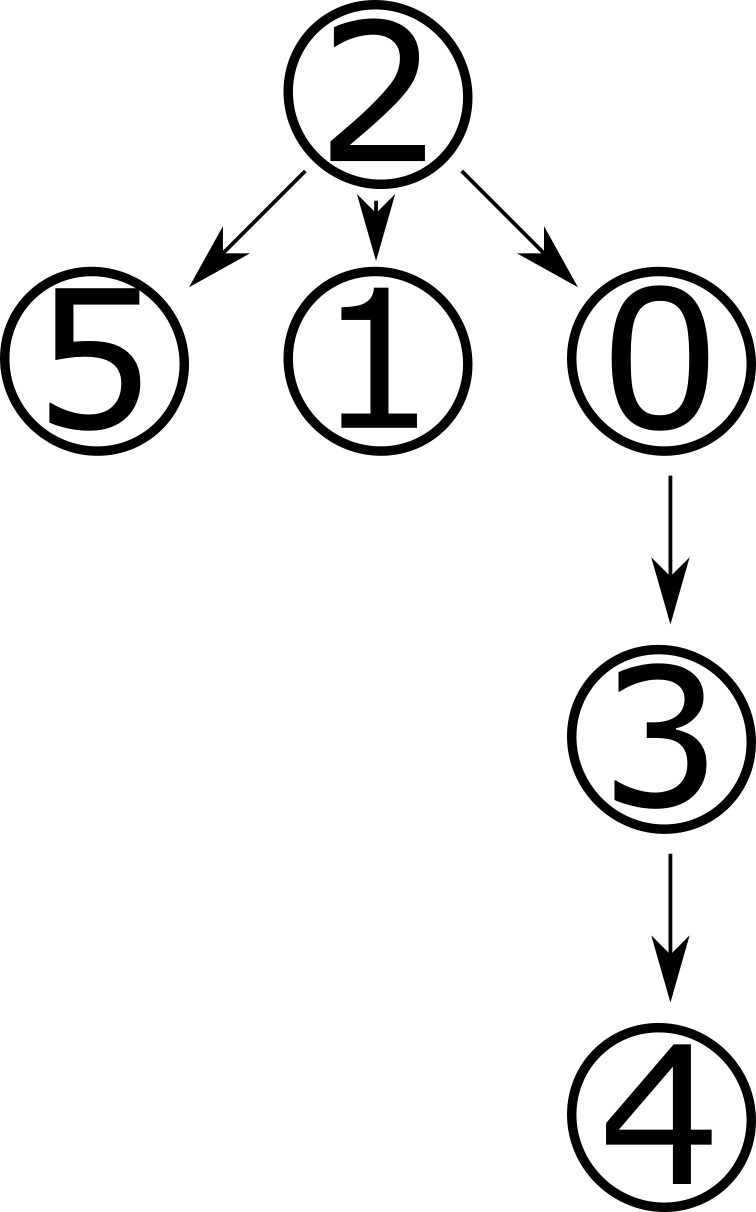
\includegraphics[scale=0.1]{IMG/PNG/28.png}
		
		\subsection{}
		
			On part donc de la liste des feuilles: 1, 6, 9, 12, 13.
			Donc dans l'ordre:
			1 est fils de 3.
			6 est fils de 10.
			9 est fils de 3 alors la liste des feuilles devient: 3, 10, 12, 13
			3 et 10 sont fils de 7.
			12 est fils de 5.
			13 est fils de 7.
			7 est fils de 5.
			
			D'où l'abre suivant:
			
			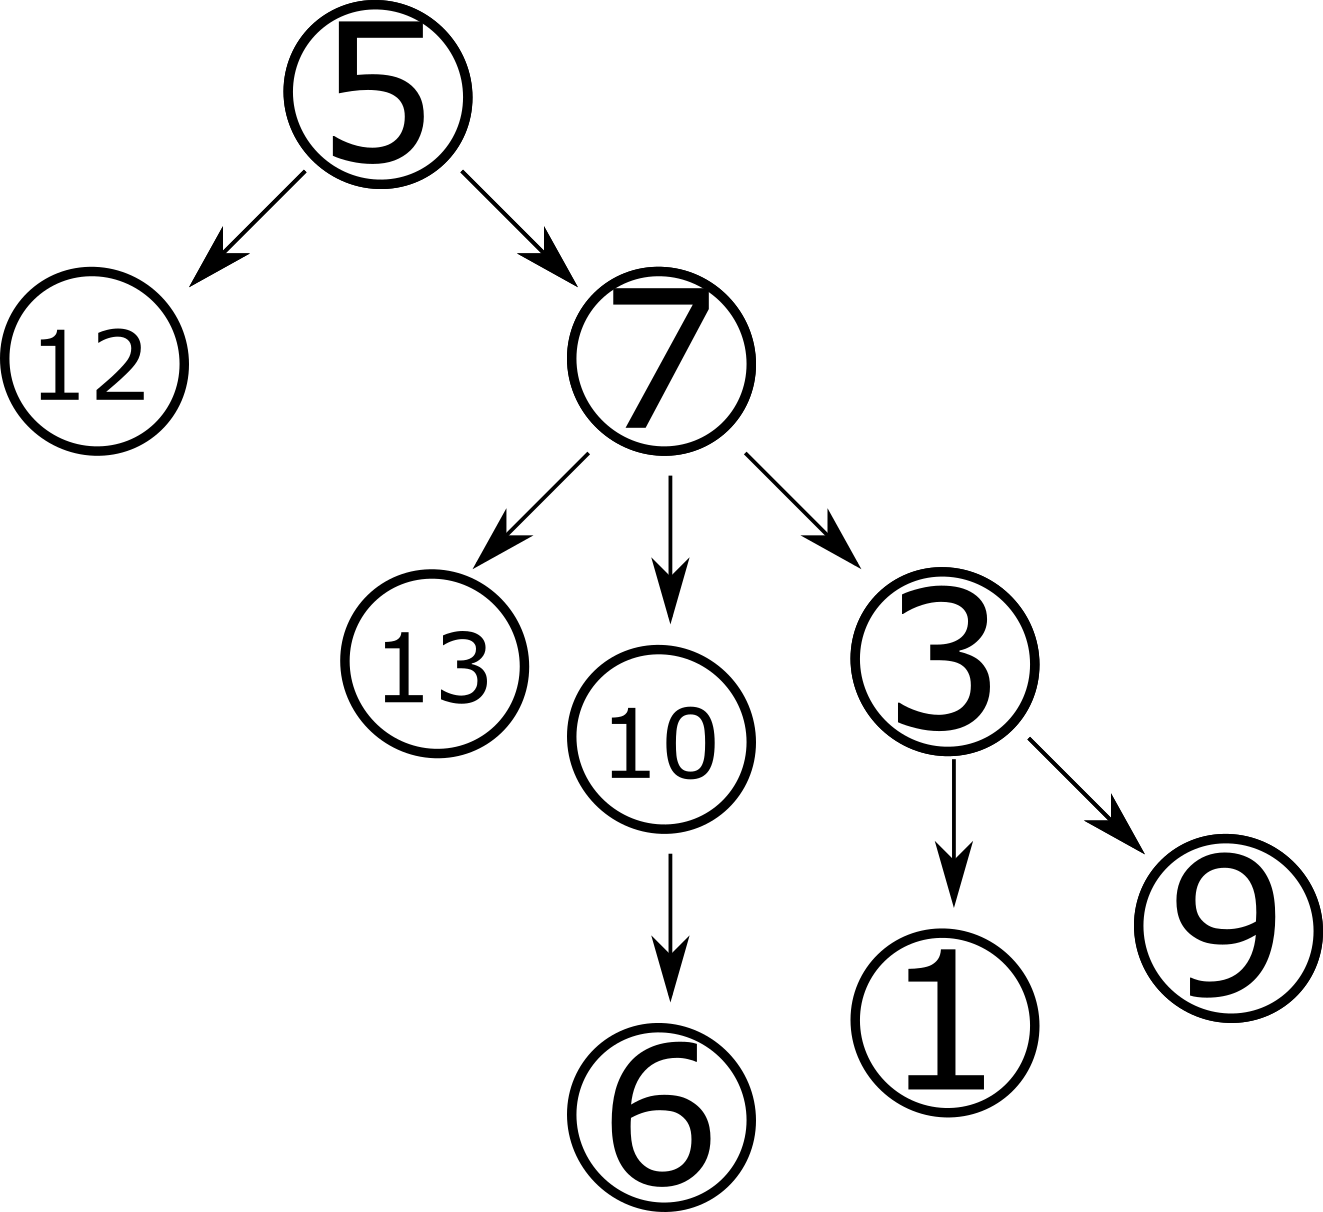
\includegraphics[scale=0.1]{IMG/PNG/29.png}
		
		\subsection{}
			
			\begin{code}
			\end{code}
		
		\subsection{}
		
		\subsection{}
		
			Par bijection on a: card $A$($E$) = card $S$($E$) = $n^{n-1}$ car cela revient à un tirage successifs avec remise de $n - 1$ éléments dans un ensemble à $n$ éléments.
		
\end{document}
